\pdfoptionpdfminorversion=5
\documentclass[9pt,hyperref={pdfpagelabels=false}]{beamer}

\mode<presentation> {
    \usetheme{HHUD}
    \setbeamercovered{invisible}
}
\usepackage[ngerman]{babel}
\usepackage[utf8x]{inputenc}
\usepackage{times}
\usepackage[T1]{fontenc}
\usepackage{amsmath}
\usepackage{subfigure}
\usepackage{graphicx}
\usepackage{hyperref}
\usepackage{xmpmulti}
\usepackage{multicol}
\usepackage{appendixnumberbeamer}

% background image
\usebackgroundtemplate{
\includegraphics[width=\paperwidth]{fig/background}}
% commands for low and high decoration in frame foot
\newcommand{\footdecorationlow}{\usebackgroundtemplate{
\includegraphics[width=\paperwidth]{fig/background_small}}}
\newcommand{\footdecorationhigh}{\usebackgroundtemplate{
\includegraphics[width=\paperwidth]{fig/background}}}

% Fix build errors on debian (http://bugs.debian.org/cgi-bin/bugreport.cgi?bug=452333)
\providecommand \thispdfpagelabel[1]{} {}

%% Die folgenden Zeilen können auskommentiert werden, um vor jedem Kapitel eine Gliederungsfolie einzufügen
% \AtBeginSection[] {
%   \footdecorationhigh
%   \begin{frame}<beamer>
%     \thispagestyle{empty}
%     \frametitle{Gliederung}
%     \vspace{-5mm}
%     \tableofcontents[currentsection]
%   \end{frame}
%   \footdecorationlow
% }

% % % % % % % % % %  CHANGE TOPIC AND AUTHOR INFORMATION HERE % % % % % % % % %
\newcommand{\abschluss}{Bachelor}                              % HIER UNZUTREFFENDES LÖSCHEN
\title{\abschluss{}arbeit:\\Secure Program Execution\\Sichere Programmausführung}                      % HIER DEN TITEL DER ARBEIT EINTRAGEN
\author{Dorian Eikenberg}                                                       % HIER DEN NAMEN UND VORNAMEN EINTRAGEN
\date{04.09.2014}                                                                % HIER DAS PRÄSENTATIONSDATUM EINTRAGEN
% % % % % % % % % % % % % % % % % % % % % % % % % % % % % % % % % % % % % % % %
\institute{Institut für Informatik\\Heinrich-Heine-Universität Düsseldorf}
\subject{Informatik}

%
% Hier beginnt das Dokument
%
\begin{document}

  \footdecorationhigh
  \begin{frame}
    \thispagestyle{empty}
    \titlepage
  \end{frame}

%  \begin{frame}
%    \thispagestyle{empty}
%    \frametitle{Gliederung}
%    \vspace{-5mm}
%    \tableofcontents
%  \end{frame}
  \footdecorationlow

  % % % % % % % % % % Ab hier werden die LaTeX-Dateien der einzelnen Abschnitte eingefügt % % % % % % % % % %

  \section{Motivation}

\begin{frame}
  \frametitle{Motivation}
  \begin{itemize}
  \item Ziel: Schutz vor nicht vertrauenswürdigen Programmen
  \begin{itemize}
   \item Testumgebung
   \item unbekannte Programme
   \item Sicherheit für Server
  \end{itemize}
  \item sicheres, automatisches Testen der C-Projekte in Informatik 2
  \end{itemize}
\end{frame}


\begin{frame}
  \frametitle{Lösungen}
  \begin{itemize}
    \item{Virtual Machine}
    \begin{itemize}
      \item{Emulation von Hardware}
      \item{separates Betriebssystem}
    \end{itemize}
    \item{Ptrace}
    \begin{itemize}
      \item{überwacht System Calls}
    \end{itemize}
    \item{Container Virtualization}
    \begin{itemize}
      \item separates Datenset
      \item nutzt den Host-Kernel
      \item isoliert durch Kernel-Funktionen
    \end{itemize}
  \end{itemize}
\end{frame}


\section{Grundlagen}

\begin{frame}
  \frametitle{Linux Containers (Lxc)}
  \begin{itemize}
    \item leichtgewichtig
    \begin{itemize}
      \item Erstellung etwa 10s
      \item Start/Stop etwa 1s
      \item Speicherverbrauch im Leerlauf etwa 3MB
    \end{itemize}
    \pause
    \item existieren als \textit{rootfs} auf dem Host System
    \begin{itemize}
      \item rootfs enthält sämtliche Dateien zur Ausführung eines Betriebssystems
      \item Ausnahme in Lxc: Kernel
    \end{itemize}
    \pause
    \item isoliert auszuführende Programme vom Rest des Systems durch:
    \begin{itemize}
      \item Chroot
      \item Kernel Namespaces (PID, mount...)
      \item Cgroups (memory, cpu...)
      \item Linux Capabilities (cap\_sys\_boot, cap\_sys\_chroot)
      \item Linux Security Modules
      \item Seccomp Policies
    \end{itemize}
  \end{itemize}
\end{frame}
  
  \section{Daemon}


\begin{frame}
  \frametitle{Zweck}
  \begin{itemize}
   \item \textit{Lxc} benötigen root-Rechte
   \item Nutzung sollte idealerweise unprivilegiert ablaufen
   \item Erstellung und Verwaltung durch einen \textit{daemon}
  \end{itemize}
\end{frame}


\begin{frame}[fragile]
 \frametitle{Daemon Design}
 \begin{itemize}
  \item Kommunikation via Socket (Unix Domain Socket)
  \item Zugriffskontrolle über Berechtigung
  \item request:\\\begin{verbatim}
	{"action": "run_prog"
	 "b64_data": program
	 "timeout": 60}
        \end{verbatim}

  \item Daemon benutzt eigenes Konfigurations-Template
  \begin{itemize}
   \item Cgroup Limits
   \item Alle Kernel Capabilities ablegen
   \item Mountpoints
  \end{itemize}
  \item Erstellt Debian Container
 \end{itemize}
\end{frame}


\begin{frame}
 \frametitle{Workflow}
 \begin{center}
  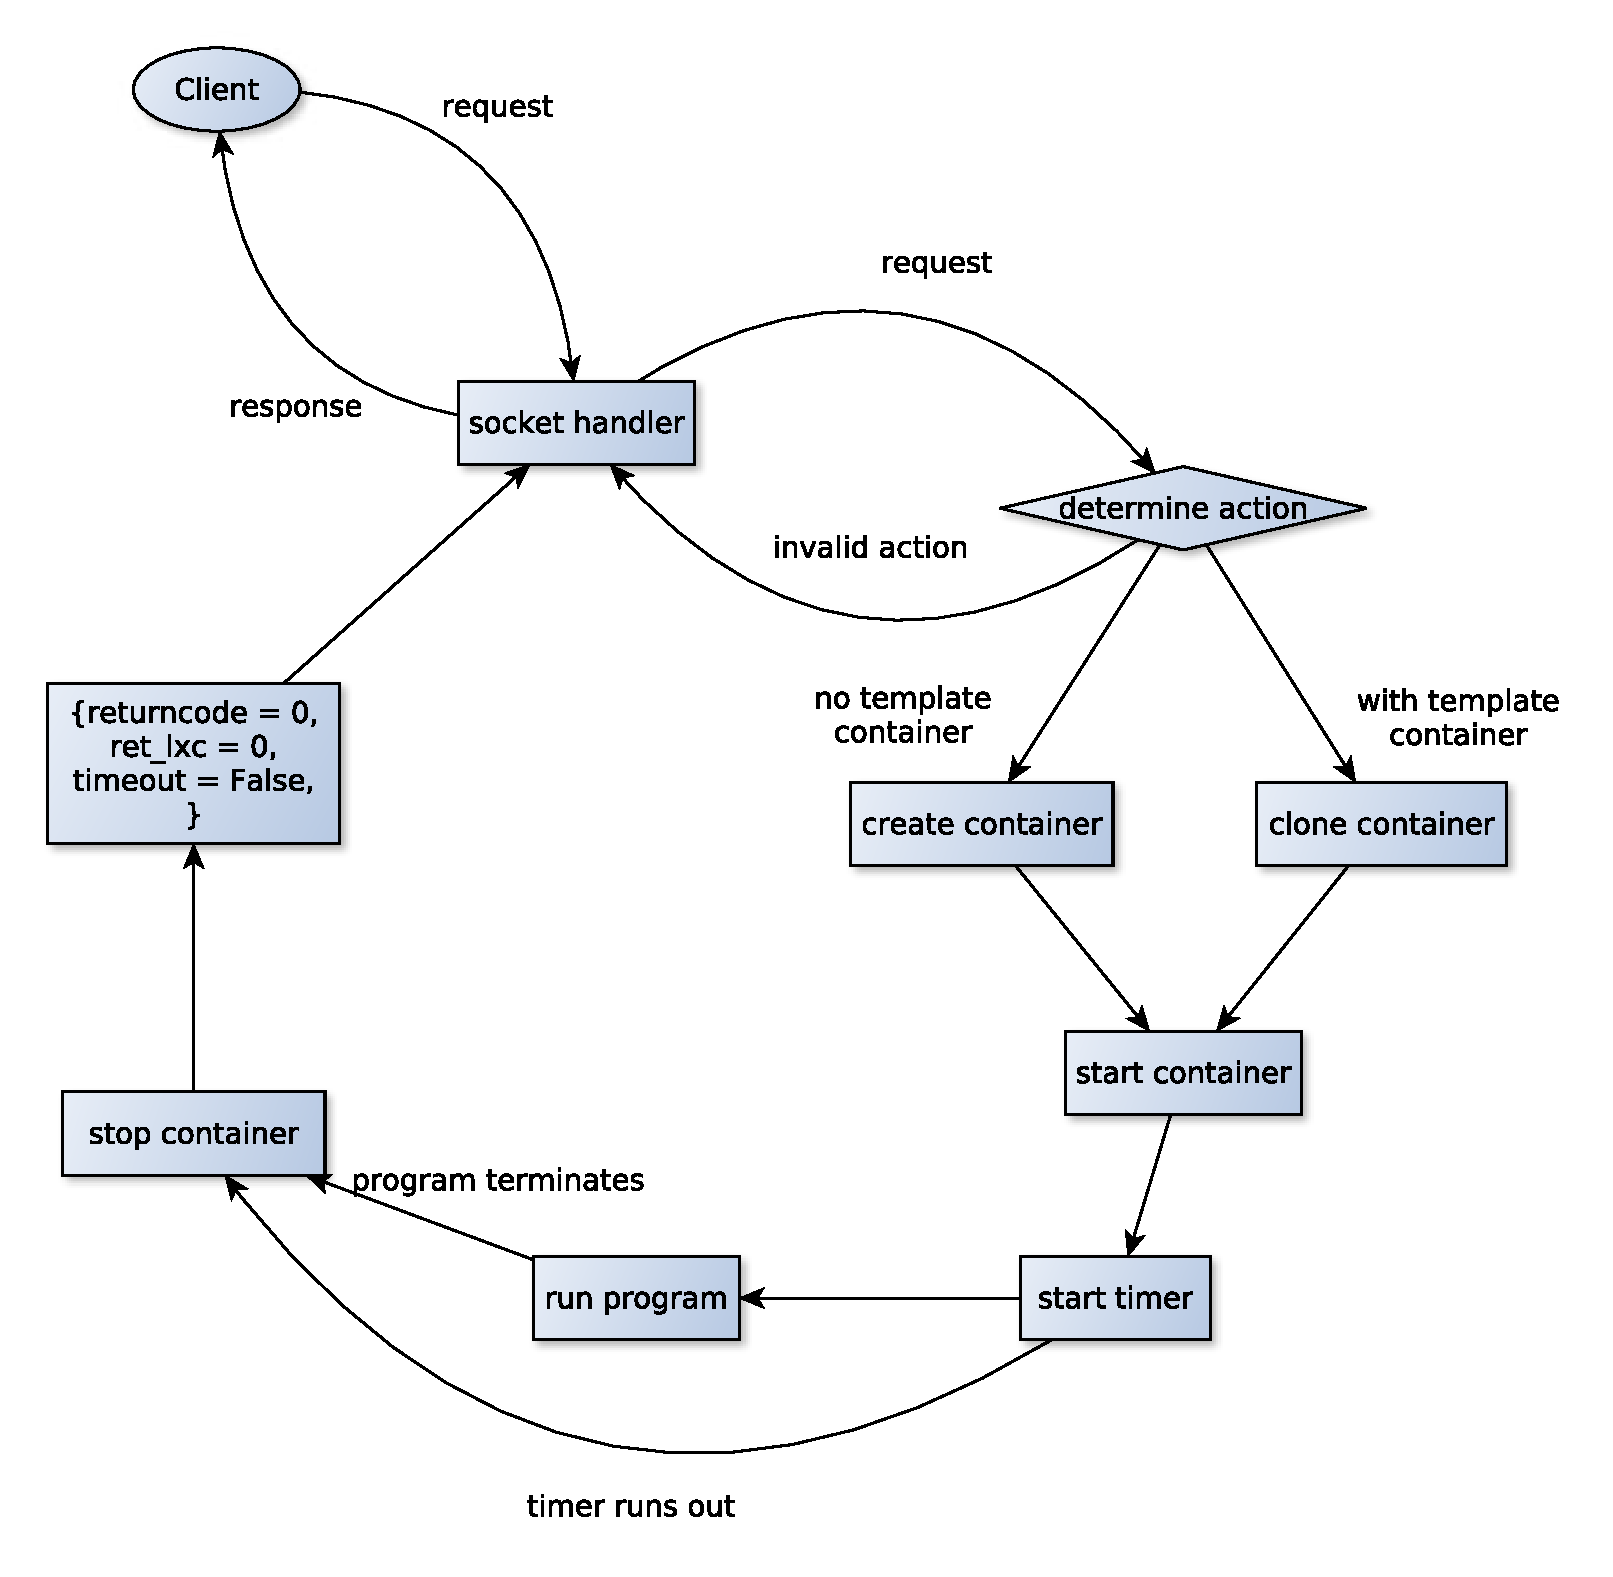
\includegraphics[width=0.7\textwidth]{fig/workflow}
 \end{center}
\end{frame}

\section{Probleme}

\begin{frame}
 \frametitle{Probleme}
 \begin{itemize}
  \item Umstrukturierung der Konfigurationsdateien
  \begin{itemize}
   \item Auslagerung von Sektionen in allgemeine Konfigurationen
   \item Änderungen an der Mountpoint Syntax
  \end{itemize}
  \item Änderungen am Rückgabewert des ausgeführten Programmes
  \item Fehlen von Kernel Modulen in Arch Linux:
  \begin{itemize}
   \item User Namespace (Befürchtung kritischer Bugs)
   \item Cgroups: Kernel Memory Extension (Memory Reclaim fehlt)
  \end{itemize}
 \end{itemize}
\end{frame}

\begin{frame}[fragile]
 \frametitle{Bug im Python Language Binding}
 \begin{itemize}
  \item API greift auf C-Funktionen zu
  \item Global Interpreter Lock
  \begin{itemize}
   \item blockt alle anderen Threads beim Ausführen einer externen C-Funktion
  \end{itemize}
  \item Timer-Thread geblockt während Programmausführung
 \end{itemize}
 Patch:
 \begin{verbatim}
       if (wait) {
+        Py_BEGIN_ALLOW_THREADS
         ret = lxc_wait_for_pid_status(pid);
+        Py_END_ALLOW_THREADS
         /* handle case where attach fails */
         if (WIFEXITED(ret) && WEXITSTATUS(ret) == 255)
             ret = -1;
 \end{verbatim}
\end{frame}

  
  \section{Tests}

\begin{frame}[fragile]
 \frametitle{Tests}
 Denial of Service (DoS) Tests:
 \begin{itemize}
  \item nicht terminierend
  \item beliebig hoher Speicherverbrauch
  \item volle CPU-Last
  \begin{itemize}
   \item 2 Container mit CPU-DoS-Programm
   \item einer mit, einer ohne Limit
   \item Beschränkung auf einen Kern bei Multicore-Systemen (cgroups)
  \end{itemize}
  \pause
  \item Fork Bomb (erzeugt rekursiv Kind-Prozesse)
 \end{itemize}
 \begin{verbatim}
  bomb() {
  bomb | bomb &
  }; bomb 
 \end{verbatim}
 \pause
 Capability Test:
 \begin{itemize}
  \item Ausgabe einer Liste mit vorhandenen Capabilities
  \item $<$Label$>$: $<$Wert$>$
 \end{itemize}
\end{frame}


  \section{Zusammenfassung/Ausblick}

\begin{frame}
  \frametitle{Zusammenfassung}
  \begin{itemize}
   \item Daemon entwickelt
   \item Tests
   \begin{itemize}
    \item Programme zum automatischen Testen entwickelt
   \end{itemize}
  \end{itemize}
\end{frame}

\begin{frame}
 \frametitle{Ausblick}
 \begin{itemize}
  \item unprivilegierte Container
  \item Daemon um Actions erweitern
  \item Mail Server
  \item Ptrace und Virtual Machines untersuchen
 \end{itemize}

\end{frame}


  % % % % % % % % % % Ende der eingefügten LaTeX-Dateien % % % % % % % % % %

\end{document}

%
% Hier endet das Dokument
%